\documentclass[11pt]{article} 
\usepackage[english]{babel}
\usepackage[utf8]{inputenc}
\usepackage[margin=0.5in]{geometry}
\usepackage{amsmath}
\usepackage{amsthm}
\usepackage{amsfonts}
\usepackage{amssymb}
\usepackage[usenames,dvipsnames]{xcolor}
\usepackage{graphicx}
\usepackage[siunitx]{circuitikz}
\usepackage{tikz}
\usepackage[colorinlistoftodos, color=orange!50]{todonotes}
\usepackage{hyperref}
\usepackage[numbers, square]{natbib}
\usepackage{fancybox}
\usepackage{epsfig}
\usepackage{soul}
\usepackage[framemethod=tikz]{mdframed}
\usepackage[shortlabels]{enumitem}
\usepackage[version=4]{mhchem}
\usepackage{multicol}

\usepackage{mathtools}
\usepackage{comment}
\usepackage{enumitem}
\usepackage[utf8]{inputenc}
\usepackage[linesnumbered,ruled,vlined]{algorithm2e}
\usepackage{listings}
\usepackage{color}
\usepackage[numbers]{natbib}
\usepackage{subfiles}
\usepackage{tkz-berge}


\newtheorem{prop}{Proposition}[section]
\newtheorem{thm}{Theorem}[section]
\newtheorem{lemma}{Lemma}[section]
\newtheorem{cor}{Corollary}[prop]

\theoremstyle{definition}
\newtheorem{definition}{Definition}

\theoremstyle{definition}
\newtheorem{required}{Problem}

\theoremstyle{definition}
\newtheorem{ex}{Example}

\tikzset{
    vertex/.style={circle,draw,minimum size=16,inner sep=0pt,font=\normalsize},
    edgelabel/.style={rectangle,draw=none,font=\footnotesize,outer sep=0pt},
    every node/.style={vertex},
    every edge quotes/.append style={edgelabel},
    every to/.append style={every node/.style={edgelabel}},
    wide/.style={line width=4pt},
    directed/.style={arrows={-Stealth[length=7pt]},font=\small},
    }


\setlength{\marginparwidth}{3.4cm}
%#########################################################

%To use symbols for footnotes
\renewcommand*{\thefootnote}{\fnsymbol{footnote}}
%To change footnotes back to numbers uncomment the following line
%\renewcommand*{\thefootnote}{\arabic{footnote}}

% Enable this command to adjust line spacing for inline math equations.
% \everymath{\displaystyle}

% _______ _____ _______ _      ______ 
%|__   __|_   _|__   __| |    |  ____|
%   | |    | |    | |  | |    | |__   
%   | |    | |    | |  | |    |  __|  
%   | |   _| |_   | |  | |____| |____ 
%   |_|  |_____|  |_|  |______|______|
%%%%%%%%%%%%%%%%%%%%%%%%%%%%%%%%%%%%%%%

\title{
\normalfont \normalsize 
\textsc{CSCI 3104 Fall 2021 \\ 
Instructors: Profs. Grochow and Waggoner} \\
[10pt] 
\rule{\linewidth}{0.5pt} \\[6pt] 
\huge Final- Standard 11 \\
\rule{\linewidth}{2pt}  \\[10pt]
}
%\author{Your Name}
\date{}

\begin{document}
\definecolor {processblue}{cmyk}{0.96,0,0,0}
\definecolor{processred}{rgb}{200, 0, 0}
\definecolor{processgreen}{rgb}{0, 255, 0}
\DeclareGraphicsExtensions{.png}
\DeclareGraphicsExtensions{.gif}
\DeclareGraphicsExtensions{.jpg}

\maketitle


%%%%%%%%%%%%%%%%%%%%%%%%%
%%%%%%%%%%%%%%%%%%%%%%%%%%
%%%%%%%%%%FILL IN YOUR NAME%%%%%%%
%%%%%%%%%%AND STUDENT ID%%%%%%%%
%%%%%%%%%%%%%%%%%%%%%%%%%%
\noindent
Due Date \dotfill Dec / $15^{th}$ / 2021 \\
Name \dotfill \textbf{Michael Ghattas} \\
Student ID \dotfill \textbf{109200649} \\


\tableofcontents

\section{Instructions}
 \begin{itemize}
	\item The solutions \textbf{should be typed}, using proper mathematical notation. We cannot accept hand-written solutions. \href{http://ece.uprm.edu/~caceros/latex/introduction.pdf}{Here's a short intro to \LaTeX.}
	\item You should submit your work through the \textbf{class Canvas page} only. Please submit one PDF file, compiled using this \LaTeX \ template.
	\item You may not need a full page for your solutions; pagebreaks are there to help Gradescope automatically find where each problem is. Even if you do not attempt every problem, please submit this document with no fewer pages than the blank template (or Gradescope has issues with it).

	\item You \textbf{may not collaborate with other students}. \textbf{Copying from any source is an Honor Code violation. Furthermore, all submissions must be in your own words and reflect your understanding of the material.} If there is any confusion about this policy, it is your responsibility to clarify before the due date. 

	\item Posting to \textbf{any} service including, but not limited to Chegg, Discord, Reddit, StackExchange, etc., for help on an assignment is a violation of the Honor Code.

	\item You \textbf{must} virtually sign the Honor Code (see Section \ref{HonorCode}). Failure to do so will result in your assignment not being graded.
\end{itemize}


\section{Honor Code (Make Sure to Virtually Sign)} \label{HonorCode}

\begin{required}
\noindent 
\begin{itemize}
\item My submission is in my own words and reflects my understanding of the material.
\item I have not collaborated with any other person.
\item I have not posted to external services including, but not limited to Chegg, Discord, Reddit, StackExchange, etc.
\item I have neither copied nor provided others solutions they can copy.
\end{itemize}

%\noindent In the specified region below, clearly indicate that you have upheld the Honor Code. Then type your name. 
\end{required}

\begin{proof}[I agree to the above, Michael Ghattas.]
%% Typing "I agree to the above," followed by your name is sufficient.
\end{proof}

\newpage
\section{Standard 11- Network Flows: Reductions}

\begin{required} \label{Problem2}
In attempting to rally allies to the Separatist cause, Count Dooku invites diplomatic parties from each of $n$ planets to a gathering on Geonosis. The $i$th diplomatic party has $p_{i} \geq 1$ members, all coming from planet $i$. Count Dooku has $m$ tables, where table $j$ has $s_{j}$ seats. In order to strengthen diplomatic ties, Count Dooku wishes to seat \textbf{all} the diplomats, so that no two diplomats from the same planet are at the same table. \\

\noindent \textbf{Example:} Suppose there are diplomatic parties from two planets, where the first party has $p_{1} = 3$ people, and the second party has $p_{2} = 2$ people. Suppose there are now \textbf{three tables} where the first table has $s_{1} = 3$ chairs, the second table has $s_{2} = 2$ chairs, and the third table has $2$ chairs. We may then set two diplomats (one from Planet 1 and one from Planet 2) at the first table, and another two diplomats (one from Planet 1 and one from Planet 2) at the second table. The remaining diplomat from Planet 1 is left at the third table.


\begin{enumerate}[label=(\alph*)]
\subsection{Problem 2a}
\item \label{2a} Describe how to reduce the above problem to the (one-source, one-sink) max-flow problem from class. Your description should be \textbf{general}, and not tied to a specific example. (You may illustrate with an example for expository purposes, but an example alone is not sufficient. E.g., ``This is how my construction is performed in general. Then for example, this is how we apply the construction to the graph I selected."). \\

\begin{proof}[Answer:] \
\item Projecting the given problem onto a graph $G$, we would need a set of nodes $n = max(i)$ that represent the political parties $p_i$, and a set of nodes $m \geq n$ that represent the tables $s_j$. Each edge $p_i \to s_j$ of $G$ has a capacity of $1$. Then, we construct a flow network $H$ which has the same vertex and edges as $G$ with the addition of $s$ as the start node, $t$ as the sink node, and edges from $s$ to the $n$ nodes with each edge having the capacity of $p_i$, and edges connecting each $s_j$ to $t$ with each edge having the capacity of $s_j$.
%Your answer here
\end{proof}


\newpage 
\subsection{Problem 2b}
\item \label{2b} Suppose there are three diplomatic parties with $p_{1} = 2$, $p_{2} = 3$, and $p_{3} = 4$ members in the respective parties. Now suppose we have four tables, where $s_{1} = 3$, $s_{2} = 2$, $s_{3} = 2$, and $s_{4} = 1$. \textbf{Using your reduction}, determine if Count Dooku can seat all the diplomats, so that no two diplomats from the same planet are at the same table. Show your work, as well as your final answer. It suffices to provide the flow network at the start of the algorithm, the flow-augmenting paths,  then the saturated flow network after running the algorithm, and the final allocations of the diplomats to tables.

\begin{proof}[Answer:] \
\begin{center}
	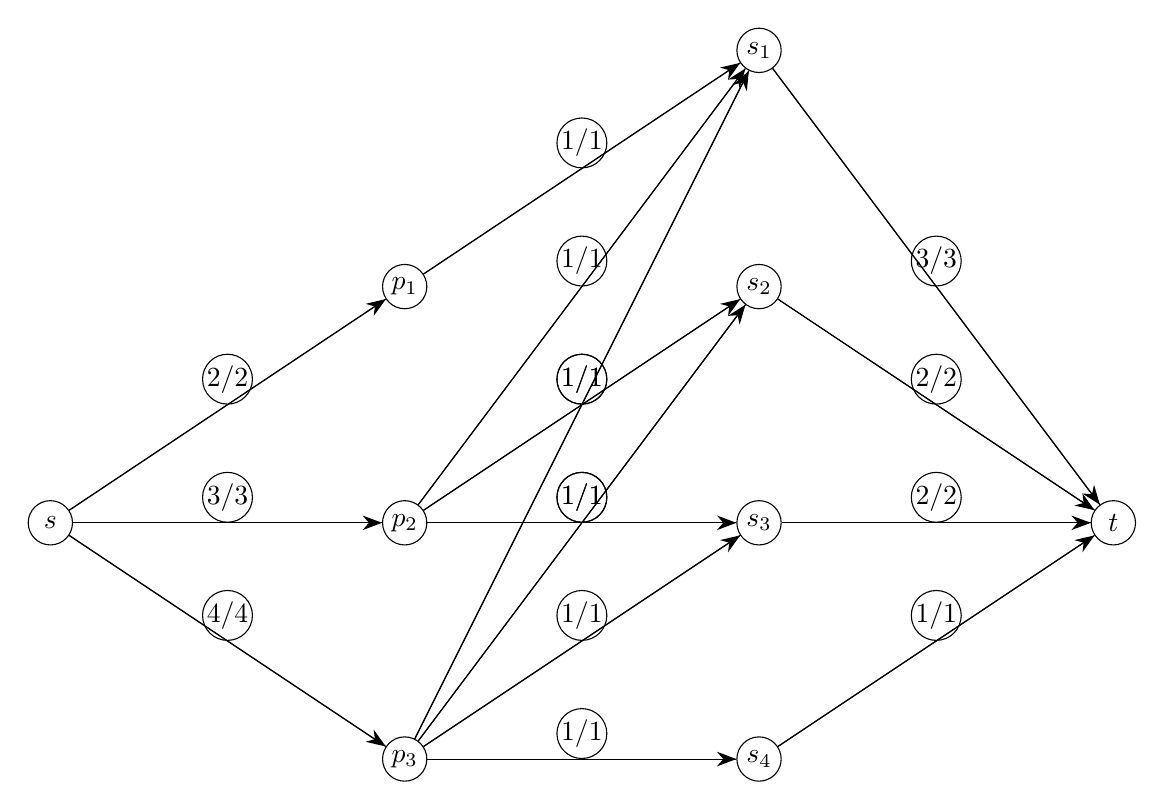
\begin{tikzpicture}[xscale=2.25,yscale=1.5]
		\node (s) at (-2,0) {$s$};
		
		\node (a) at (0,2) {$p_1$};
		\node (b) at (0,0) {$p_2$};
		\node (c) at (0,-2) {$p_3$};
		
		\node (d) at (2,2) {$s_2$};
		\node (e) at (2,0) {$s_3$};
       		 \node (f) at (2,-2) {$s_4$};
       		 \node (g) at (2,4) {$s_1$};
		 
       		 \node (t) at (4,0) {$t$};
	
	
	\draw[directed] (s) to (a);
	\draw[directed] (s) to (b);
	\draw[directed] (s) to (c);
	
	\draw[directed] (a) to (g);
	
	\draw[directed] (b) to (d);
	\draw[directed] (b) to (e);
	\draw[directed] (b) to (g);
	
	\draw[directed] (c) to (d);
	\draw[directed] (c) to (e);
	\draw[directed] (c) to (f);
	\draw[directed] (c) to (g);
	
        \draw[directed] (d) to (t);
	\draw[directed] (e) to (t);
	\draw[directed] (f) to (t);
	\draw[directed] (g) to (t);
	
        
        	\path (s) edge node[above] {$2 / 2$} (a);
        	\path (s) edge node[above] {$3 / 3$} (b);	
        	\path (s) edge node[above] {$4 / 4$} (c);	
	
        	\path (a) edge node[above] {$1 / 1$} (g);
	
        	\path (b) edge node[above] {$1 / 1$} (d);
        	\path (b) edge node[above] {$1 / 1$} (e);	
        	\path (b) edge node[above] {$1 / 1$} (g);
	
        	\path (c) edge node[above] {$1 / 1$} (d);
        	\path (c) edge node[above] {$1 / 1$} (e);	
        	\path (c) edge node[above] {$1 / 1$} (f);
        	\path (c) edge node[above] {$1 / 1$} (g);
	
        	\path (d) edge node[above] {$2 / 2$} (t);
        	\path (e) edge node[above] {$2 / 2$} (t);	
        	\path (f) edge node[above] {$1 / 1$} (t);
        	\path (g) edge node[above] {$3 / 3$} (t);	
    \end{tikzpicture}
\end{center}
\item \textbf{While we will be able to seat no more than one diplomat from each party at each table, we would not be able to seat everyone at a table since there are more diplomats than chairs. Based on our flow network above, one diplomat from $p_1$ will not be seated at all.}
%Your answer here
\end{proof}

\end{enumerate}
\end{required}

%%%%%%%%%%%%%%%%%%%%%%%%%%%%%%%%%%%%%%%%%%%%%%%%%%
\end{document} % NOTHING AFTER THIS LINE IS PART OF THE DOCUMENT



